\section{Related work}
\subsection{Internet of things}
Rob van Kranenburg defines IoT as:
\begin{quote}
    a dynamic global network infrastructure with self-configuring capabilites based on standard and interoperable communcation protocols where physical and virutal 'Things' have identites, physical attributes, and virtual parsonalites and use intelligent interfaces, and are seamlessly integrated into the information netork.  
\end{quote}

\subsection{Industry 4.0}
%Industry 4.0 definition.
Lasi \cite{Lasi2014}  argues that the term industry 4.0 was coined beforehand as a planned fourth industruial revolution.
The use of internet of things devices, IoT-devices from now on, and cyber physical systems, CPS from now on is what defines the fourth industrial revolution Vadiya means \cite{Vaidya2018}.
See figure x for a short historic overview of previous industrial revolutions. 
\begin{figure}
    \centering
    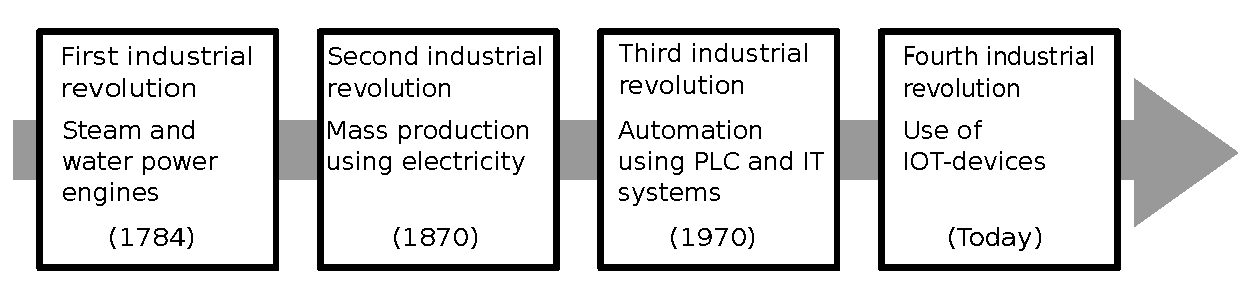
\includegraphics[width=\textwidth]{Pictures/Industrial_revolution.pdf} 
    \caption{Historic overview of previous industrial revolutions}
    \label{Indutrial revolutions}
\end{figure}

According to Vadiya \cite{Vaidya2018} industry 4.0 promotes the connection of sensors and devices both to the internet and to other sensors or devices.

%Intelligent  sensors.

Hozdić \cite{Hozdic2015} states that a sensor is a device capable of providing an appropriate output in response to a measured value.
One key feature of intelligent sensor is that in order to increase the level of information proeccesing it processes the information at a logical level Hozdić \cite{Hozdic2015} argues.
A Intelligent sensor  is capable of executing actions based on the measured value in contrast to regular sensors, making them easier to set up and use means Hozdić \cite{Hozdic2015}.

%Cyber Physical Systems (CPS).
Hozdić defines cyber physical system, CPS, as a new generation of system that integrate both physical and computer abilities. \cite{Hozdic2015}
A cyber physical system consists of two parts, one cybernetic and one physical.
The cybernetic part of the system can be viewed as a summation of logic and sensor units while the physical part of the system can be viewed as a summation of the accuator units Hozdić adds. \cite{Hozdic2015}
Xu et. al. states that cyber physical systems is a key part of Industry 4.0. In contrast to the simple embedded systems of today will be exceeded due to advances in CPS that enables enhanced capability, scalability, adaptibility, resilency, safety, usability and secruity.  \cite{Xu2018}
Hozdić argues that it is the CPS abilities to share and recieve information from intelligent sensors that connect to digital networks is what enables and form an internet of things. \cite{Hozdic2015}
 

\subsection{Arrowhead framework}
%Local cloud.
A local cloud is defined as a self contained network with at least the thrre mandatory systems deployed, more on those in a later paragrapg. 
Delsing et.al. also argues that except the three mandatory core systems running a local cloud also needs at least one application system deployed \cite{Delsing2017}.

%Service and systems.
Two terms have to be introduced in order to further understand what the Eclipse Arrowhead framework aims to accomplish, services and systems.
Delsing et. al. defines a system as what is providing or consuming a service. \cite{Delsing2017} 
Furthermore a service is defined as what is used to convey information between a provider and a consumer Delsing et. al. argues \cite{Delsing2017}

%Mandatory core systems.
The Eclipse Arrowhead framework, Arrowhead from now on, consists of three mandatory core systems according to Delsing et. al. \cite{Delsing2017}
To fully operate a local cloud as defined in the previous section it must according to Delsing \cite{Delsing2017} contain:
\begin{itemize}
    \item Service registry system.
    \item Authorization system. 
    \item Orchestration system.
\end{itemize}
%Service registry system.
The service registry system is responsibly for enabling discovery and registring services Delsing et. al. \cite{Delsing2017} states. 
According to the Eclipse Arrowhead projects own github page \cite{Github2021} the service registry system provides the database which stores the offered services in the local cloud.
The github page also states the three main objectives of the service registry system are:
\begin{itemize}
    \item To allow application system to register available services to the database. 
    \item Remove or update available services from the database.
    \item Allow application system to use the lookup functionality of the registry.
\end{itemize}
%Authorization system.
The Authorization system is contains two databases for keeping track on which system can consume services from which other system, depending on whether or not the Application system are in the same cloud or not according the projects github page \cite{Github2021}
The github documentation also states that if the authorization happens within the same cloud it is called intra-cloud authorization and if it happens accross two local clouds it is called inter-cloud authorization. \cite{Github2021} \\ \\
%Orchestrator system.
The Orchestration system is responsible for pairing and finding service providers and consumer Delsing et. al. declares. \cite{Delsing2017} 
Delsing et. al. continues to state that the orchestrator also stores the orchestration requirments and the resulting orchestration rules. \cite{Delsing2017} 
The projects documentation argues that the main objective of the orcherator system is to find an appropriate provider for the requesting consumer system. \cite{Github2021}
The documentation also states that there are two types of orchestration, store orchestration and dynamic orchestration.
Store orchestration uses the database orchestration store to find predefined orchestration rules.
Dynamic orchestration on the other hand searches the entire local cloud, or even other clouds, in order to find mathing provider. \cite{Github2021}
\subsection{Security}
\subsection{Communication} 
